% --- PROPOSED 2-TYPE MSDA METHODOLOGY ---

\noindent This chapter presents the proposed methodology in detail. The system architecture involves a complete pipeline from task generation and severity classification, through urgency scoring using an extended Analytic Hierarchy Process (AHP), to the final task assignment using an adapted 2-Type Multi-Stage Deferred Acceptance (MSDA) algorithm.

\section{Overview of the Proposed Pipeline}

The proposed system replaces the baseline M-DAFTO single-pool approach with a severity-aware matching pipeline. The pipeline operates in sequential stages to ensure that critical healthcare tasks are prioritised without entirely starving routine tasks. First, tasks are generated and classified by severity. Second, delay and energy costs are calculated and normalised. Third, a 4-criteria AHP model generates dynamic weights to compute an urgency score for each task-node pair. Finally, the adapted 2-Type MSDA algorithm uses these urgency scores to form preference lists and execute the matching process.

\section{Severity-Aware Task Classification and Quotas}

Unlike the baseline M-DAFTO algorithm which treats all tasks equally, the proposed system categorises tasks into two distinct classes based on the framework introduced by Oomori and Manabe \cite{oomori2026strategyproof}:
\begin{itemize}
\item \textbf{Major Tasks (R-type):} Critical healthcare operations, such as surgical robotic control or emergency patient monitoring.
\item \textbf{Minor Tasks (S-type):} Routine healthcare operations, such as regular data logging or non-urgent checkups.
\end{itemize}

To ensure Major tasks are never starved of computational resources during high-load scenarios, the system enforces a strict quota structure on every fog node. 
Figure~\ref{fig:quota_structure} illustrates this quota tracking mechanism. Each fog node maintains four quota values:
\begin{itemize}
\item $p_c$: minimum quota for all tasks
\item $q_c$: maximum quota for all tasks (= numberOfVRUs)
\item $pr_c$: minimum guaranteed quota for Major tasks
\item $qr_c$: maximum allowed quota for Major tasks
\end{itemize}

\begin{figure}[htbp]
\centering
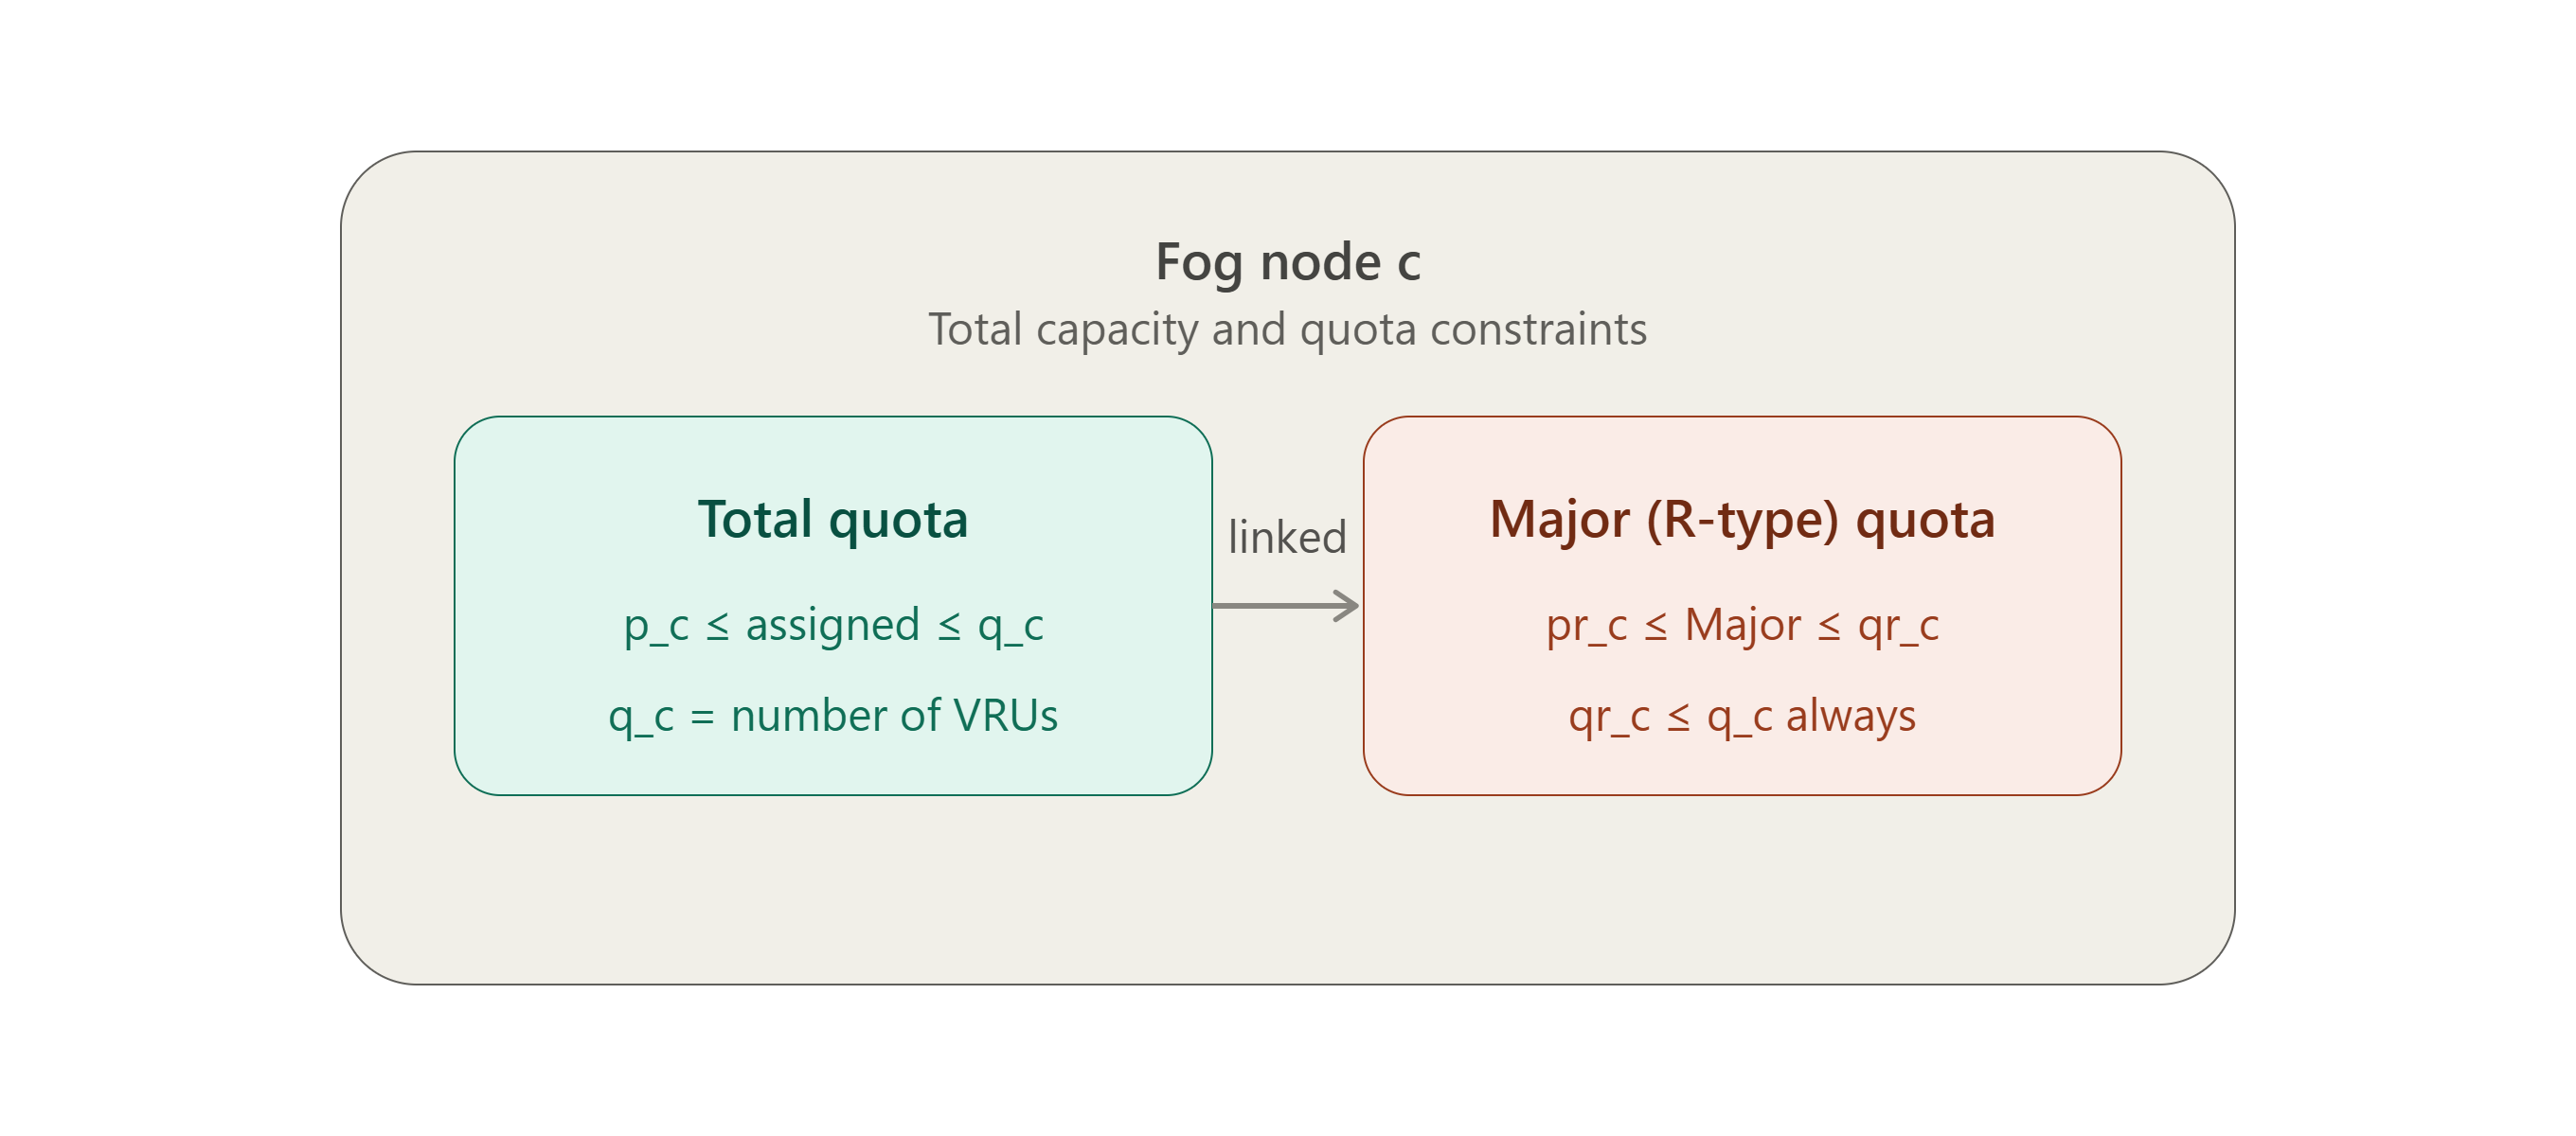
\includegraphics[width=0.85\textwidth]{Images/fog_node_quota_structure.png}
\caption{Fog node quota structure showing separate quota tracking for Major (R-type) and Minor (S-type) tasks, adapted from \cite{oomori2026strategyproof}.}
\label{fig:quota_structure}
\end{figure}

\section{The Severity-Aware 4-Criteria Urgency Model}

Before tasks can be matched to fog nodes, they must rank the fog nodes based on urgency. The baseline M-DAFTO model relies on a simple 2-criteria urgency function (delay and preference count). The proposed system introduces a novel 4-criteria model that incorporates both energy consumption and explicit severity weighting.

\subsection{Severity-Weighted Normalisation}
Delay (measured in seconds) and Energy (measured in Joules) operate on vastly different scales. A severity-weighted Min-Max normalisation is introduced to align these metrics:
\begin{equation}
\text{weight} = \begin{cases} 0.5 & \text{if severity} = \text{``Minor''} \\ 1.0 & \text{if severity} = \text{``Major''} \end{cases}
\end{equation}
\begin{align}
nd_{ij} &= \frac{\text{delay}_{ij} - \text{minDelay}}{\text{maxDelay} - \text{minDelay}} \times \text{weight} \\
ne_{ij} &= \frac{\text{energy}_{ij} - \text{minEnergy}}{\text{maxEnergy} - \text{minEnergy}} \times \text{weight}
\end{align}

\subsection{Severity Score}
To actively push Major tasks higher in the preference rankings, a severity multiplier $\gamma(T_i)$ is dynamically calculated:
\begin{equation}
\gamma(T_i) = 1 + c_i \times 0.5
\end{equation}
where $c_i = 1$ for Major tasks and $c_i = 0$ for Minor tasks. This forces $\gamma = 1.5$ for critical tasks and $\gamma = 1.0$ for routine tasks.

\subsection{4-Criteria Urgency Function and AHP}
The final urgency function $U(T_i, F_j)$ for a task $T_i$ on fog node $F_j$ is computed as:
\begin{equation}
U(T_i, F_j) = w_1 \frac{1}{\Delta d} + w_2 \frac{1}{\text{pref}(T_i)} + w_3 \frac{1}{\text{energy}_{ij}} + w_4 \gamma(T_i)
\end{equation}
where $\Delta d = \text{deadline}_i - \text{delay}_{ij}$.

The weights $w_1 \ldots w_4$ are generated using a 4$\times$4 Analytic Hierarchy Process (AHP) matrix. The weight generation process follows three rigorous steps \cite{saaty1980ahp}:

\textbf{1. Pairwise Matrix Construction (PMC):} Four random values $v[1..4]$ are drawn from $[1.0, 9.0]$. The pairwise comparison matrix $P$ is built where $P_{xy} = \text{getSaatyScale}(v_x / v_y)$ for $x < y$, with $P_{yx} = 1/P_{xy}$ and $P_{xx} = 1.0$.

\textbf{2. Column Weight Determination (CWD):} The matrix $P$ is column-normalised to produce $\bar{P}$, and the rows of $\bar{P}$ are averaged to obtain the final weights $W = [w_1, w_2, w_3, w_4]^T$.

\textbf{3. Consistency Check (CC):} 
Unlike the baseline's 2$\times$2 matrix which is trivially consistent (CR = 0 always), this 4$\times$4 matrix requires genuine consistency validation. The maximum eigenvalue $\lambda_{\max}$ is computed:
\begin{align}
\lambda_{\max} &= \text{average}\left(\frac{\text{rowSum}(P \cdot W)}{W_x}\right) \\
CI &= \frac{\lambda_{\max} - n}{n - 1}, \quad RI = 0.90 \text{ (for } n=4\text{)} \\
CR &= \frac{CI}{RI}
\end{align}
The generated weights are only accepted if $CR \leq 0.1$. Otherwise, the matrix is regenerated.

\section{The 2-Type MSDA Matching Engine}

Before executing the matching algorithm, the system must generate preference and precedence lists to dictate the order of matching, as structurally required by the MSDA framework.

\subsection{Preference and Precedence Lists}
\begin{itemize}
\item \textbf{Task Preference Lists:} During the deferred acceptance process, each task $T_i$ must propose to fog nodes in its order of preference. A task's preference list (\texttt{preferredFogIndices}) is constructed by sorting all available fog nodes in ascending order of their combined normalised cost, \texttt{normSum} ($nd_{ij} + ne_{ij}$). This ensures that tasks always propose to the most delay-and-energy efficient fog nodes first.
\item \textbf{Fog Node Preference Lists:} Each fog node $F_j$ evaluates all tasks using the 4-criteria urgency function $U(T_i, F_j)$ to determine its own preferences. It generates three separate sorted rankings: one for all tasks, one strictly for Major tasks, and one strictly for Minor tasks.
\item \textbf{Task Precedence Lists:} To determine which tasks propose first during the deferred acceptance rounds, tasks are placed into precedence lists sorted strictly by their tightest deadlines. Separate precedence lists are maintained for Major and Minor tasks.
\end{itemize}

These lists are then fed into the adapted 2-Type MSDA algorithm.

\begin{figure}[htbp]
\centering
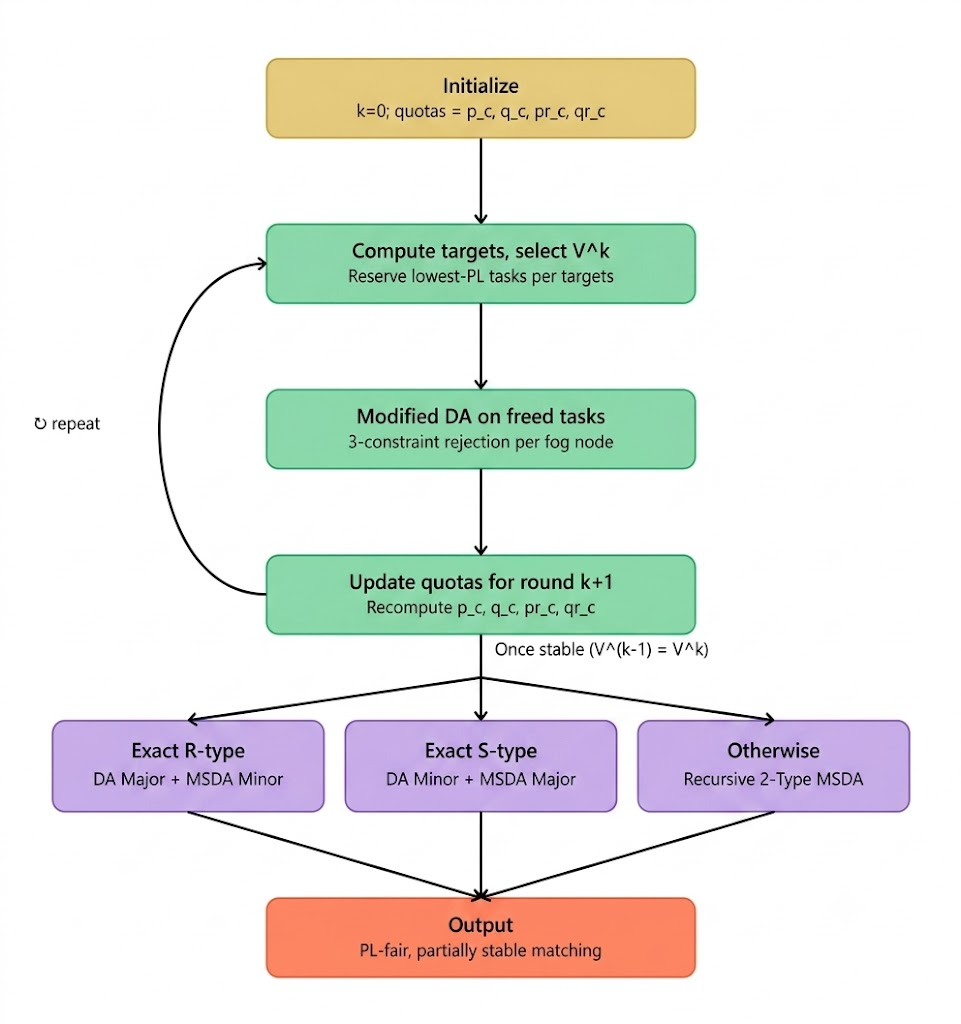
\includegraphics[width=0.95\textwidth]{Images/two_type_msda_algorithm_flow.png}
\caption{Flowchart of the adapted 2-Type MSDA matching engine, adapted from \cite{oomori2026strategyproof}.}
\label{fig:algorithm_flow}
\end{figure}

The matching engine utilises a Modified Deferred Acceptance (Modified DA) sub-routine. As shown in Algorithm \ref{alg:modified_da}, this routine simultaneously enforces the strict Major and Minor capacity constraints defined by the fog node quotas.

\begin{algorithm}[htbp]
\caption{Modified Deferred Acceptance (Fog Node Receiver Logic)}
\label{alg:modified_da}
\begin{algorithmic}[1]
\REQUIRE New proposal from task $T_i$ to Fog Node $F_j$
\vspace{1.5mm}
\STATE \textbf{Action:} $F_j$ tentatively accepts $T_i$.
\STATE \textbf{Constraint Checks:}
\WHILE{$F_j$ violates any constraint}
    \IF{Accepted Major tasks $> qr_c$}
        \STATE Reject the lowest-ranked \textbf{Major} task currently held by $F_j$.
    \ENDIF
    \IF{Accepted Minor tasks $> q_c - pr_c$}
        \STATE Reject the lowest-ranked \textbf{Minor} task currently held by $F_j$.
    \ENDIF
    \IF{Total accepted tasks $> q_c$}
        \STATE Find lowest-ranked Major task ($M_{worst}$) and Minor task ($m_{worst}$).
        \STATE Reject whichever is ranked lower overall between $M_{worst}$ and $m_{worst}$.
    \ENDIF
\ENDWHILE
\end{algorithmic}
\end{algorithm}

\newpage
The outer loop of the matching engine handles the multi-stage quota enforcement, mathematically defined in Algorithm \ref{alg:two_type_msda}. To formally track the assignment process across multiple iterations, the following notations are introduced:
\begin{itemize}
\item $k$: The current iteration index of the multi-stage algorithm.
\item $V^k$: The set of active tasks making proposals during iteration $k$.
\item $vs^k, vr^k, vt^k$: The aggregated target minimum quotas remaining across all fog nodes for Minor tasks, Major tasks, and all tasks combined, respectively, at iteration $k$.
\item $\mu^k$: The tentative matching outcome resulting from the Modified DA execution in iteration $k$.
\item $p_j^k, q_j^k, pr_j^k, qr_j^k$: The dynamically updated remaining quotas for fog node $F_j$ at iteration $k$.
\end{itemize}

By iteratively tightening the active set of tasks $V^k$ based on the remaining aggregate quotas, the engine guarantees that Major tasks secure their minimum quotas $pr_j$ without exceeding their strict ceilings $qr_j$. Once targets are met, the algorithm recursively branches to execute standard DA or MSDA for the remaining subgroups.

\begin{algorithm}[htbp]
\caption{Adapted 2-Type MSDA Algorithm}
\label{alg:two_type_msda}
\begin{algorithmic}[1]
\STATE Set $k = 0$, $V^0 = T$, $p_j^1 = p_c$, $q_j^1 = q_c$, $pr_j^1 = pr_c$, and $qr_j^1 = qr_c$ for all $F_j \in F$.
\REPEAT
    \STATE $k = k + 1$
    \STATE Let $vs^k = \sum_{F_j \in F} \max(0, p_j^k - qr_j^k)$, $vr^k = \sum_{F_j \in F} pr_j^k$, and $vt^k = \sum_{F_j \in F} p_j^k$.
    \STATE Set $V^k$ be the minimum set of tasks with the lowest priority according to $\succ$ which satisfies $|V^k| \geq vt^k$, $|V^k \cap T_{Minor}| \geq vs^k$, and $|V^k \cap T_{Major}| \geq vr^k$.
    \IF{$V^{k-1} \setminus V^k \neq \emptyset$}
        \STATE Execute Modified DA (Algorithm \ref{alg:modified_da}) on the tasks in $V^{k-1} \setminus V^k$. Let $\mu^k$ be the matching in this round.
        \FOR{each $F_j \in F$}
            \STATE $q_j^{k+1} = q_j^k - |\mu^k(F_j)|$,
            \STATE $qr_j^{k+1} = \min(qr_j^k - |\mu^k(F_j) \cap T_{Major}|, q_j^{k+1})$,
            \STATE $pr_j^{k+1} = \max(0, pr_j^k - |\mu^k(F_j) \cap T_{Major}|)$, and
            \STATE $p_j^{k+1} = \max(0, p_j^k - |\mu^k(F_j) \cap T_{Minor}| - \max(pr_j^k, |\mu^k(F_j) \cap T_{Major}|)) + pr_j^{k+1}$.
        \ENDFOR
    \ELSE
        \STATE Let $F' (\subseteq F)$ be the set of fog nodes which satisfies $p_j^k > 0$.
        \IF{$|V^k \cap T_{Major}| == vr^k$}
            \STATE Execute Standard DA on $V^k \cap T_{Major}$ and every fog node $F_j \in F'$ with $pr_j = qr_j = qr_j^k$. (For other $F_{j'} \notin F'$, set $pr_{j'} = qr_{j'} = 0$.)
            \STATE Execute Single-Type MSDA on $V^k \cap T_{Minor}$ with $p_j = p_j^k - pr_j^k$ and $q_j = q_j^k - pr_j^k$ for $F_j \in F'$ and $p_{j'} = 0$, $q_{j'} = q_{j'}^k$ for $F_{j'} \notin F'$.
            \STATE \textbf{exit} /* end of the algorithm */
        \ELSIF{$|V^k \cap T_{Minor}| == vs^k$}
            \STATE Execute Standard DA on $V^k \cap T_{Minor}$ and every fog node $F_j \in F'$ with $p_j = q_j = \max(p_j^k - qr_j^k, 0)$. (For other $F_{j'} \notin F'$, set $p_{j'} = q_{j'} = 0$.)
            \STATE Execute Single-Type MSDA on $V^k \cap T_{Major}$ with $pr_j = pr_j^k$ and $qr_j = qr_j^k$ for $F_j \in F'$ and $pr_{j'} = 0$, $qr_{j'} = qr_{j'}^k$ for $F_{j'} \notin F'$.
            \STATE \textbf{exit} /* end of the algorithm */
        \ELSE
            \STATE /* $|V^k \cap T_{Major}| > vr^k$ and $|V^k| == vt^k$ */
            \STATE Execute Adapted 2-Type MSDA on tasks in $V^k$ and every fog node $F_j \in F'$ with $pr_j = p_j = pr_j^k$, $qr_j = \min(qr_j^k, p_j^k)$, and $q_j = p_j^k$. (For other $F_{j'} \notin F'$, set $p_{j'} = q_{j'} = pr_{j'} = qr_{j'} = 0$.)
            \STATE \textbf{exit} /* end of the algorithm */
        \ENDIF
    \ENDIF
\UNTIL{forever}
\end{algorithmic}
\end{algorithm}

\section{Algorithmic Complexity}
A single Deferred Acceptance round has a complexity of $O(T \times F)$ where $T$ is the number of tasks and $F$ is the number of fog nodes. The MSDA stages are inherently bounded by $T$ because each stage successfully matches at least one task or exhausts a quota. Therefore, the worst-case overall complexity is $O(T^2 \times F)$. In practice, convergence is significantly faster because the tight quota constraints limit the number of required matching stages. The Modified DA adds a negligible constant-factor overhead for enforcing the three simultaneous constraints.
